\documentclass{book}
\usepackage{graphicx} %for importing pictures
\usepackage{float}
\usepackage{alltt} %extended verbatim mode
\usepackage{fullpage}
\renewcommand{\ttdefault}{txtt} %bold in alltt

\begin{document}
\title{ESP Design Document}
\author{Nathan Alday}
\date{\today}
\maketitle

\chapter{Philosophy}
\section{Introduction}
ESP is intended to be a educational simulation framework that focuses on being easy to both use and understand at the source level for undergraduate level students and more advanced users. ESP is intended to be primarily a teaching tool that also provides a universally available modelling and simulation toolbox that is both effective and accessible for real world applications.

\section{Objectives}
ESP's design objectives are, in order:
\begin{description}
	\item[Pedagogy] The primary purpose of ESP to teach how modelling and simulation works, how to apply good programming and documenting practices to modeling and simulation projects and how to actually write/modify simulations.
	\item[Utility/Hackability/Accessibility] After pedagogy, utility is ESP next highest goal. To maximize its utility, a modeling and simulation code must usefully address a wide variety real world problems. It must also be easily modified and extended to fit the user's needs. And it must be accessible, both from an ease of use standpoint and easily obtained.
	\item[Accuracy] The code should be as bug free as possible and the results should be as accurate as possible.
	\item[Scalability] ESP must be easily scalable to utilize and demonstrate the power of distributed computing as well as teach the principles of designing scalable modelling and simulation software. This includes being scalable across both processors and computers.
	\item[Performance] ESP should be as performant as possible while still meeting the higher objectives.
\end{description}

To best meet these objectives, ESP must be open source and written primarily in an accessible, powerful language that easily interfaces with other languages. We choose Python for its batteries included approach, growing popularity in the modelling and simulation domain, ease of use and accessibility, cross platform portability and large and well supported open source projects and community.

\section{Design Overview}

For pedagogy, modifiability and scalability, ESP must be modular both at the process level and at the module and function levels. As a result, the framework will consist of three distinct parts, each of which has a corresponding Python module (in parentheses): the numerical and modelling libraries (libs), a process level intermodel  coordination program (controller) and a set of data visualization, data references and analysis utilities (utils). 

Additionally, clear documentation, particularly of the numerical and modelling libraries, is a central part of the design. The code and its comments should clearly explain and demonstrate each model and numerical method. Furthermore, each model and numerical method as well as each class and function exposed in the libs API should have a corresponding document explaining its functionality and how and why it is used in a pedagogical fashion. Most likely, this will be in a wiki format.

To maximize utility, interfaces for the numerical and modelling libraries will be provided in as many languages as is practical.

\subsection{The Numerical and Modelling Libraries}

The numerical and modelling libraries are the core of ESP. They will implement both numerical routines such as linear algebra routines, integrators, useful numerical types, system solvers and optimizers as well as simulation models such as aerodynamics models, finite element models and logistics models.

The each model will be accessible through at least three submodules, each with a different tradeoff between the pedagogy, accessibility and performance.

\begin{description}
	\item[standard] The standard module is the canonical module. All numerical routines and models in ESP will have an actual implementation in the standard module. Its sole objective is to teach through demonstration both how to implement a routine or model and how it works. Clarity, accesssibility, correctness and modularity take precedence over performance. Routines and models in the standard module should have no dependencies other than the Python interpretter and its default modules.  They should also be as type agnostic as possible (i.e. able to operate on multiple classes in the numeric hierarchy such as decimal and float as well as external types such as mpmath's mp and iv types). The explanation of routines and modules in the documentation should focus on the standard module implementations.
	\item[fast] The fast module should consist of reimplementations of the routines and models from the standard module with a greater emphasis on performance. Written with an emphasis of performance over clarity, routines and models should still be written in pure Python, but may use outside, easily accessible and open source pure Python dependencies (like mpmath and numpy) while maintaining an API that matches the standard module API, but may contain extra keyword and variable length arguments. Routines and models that haven't been reimplemented should remain accessible through the fast module and simple call their standard model versions. 
	\item[faster] The faster module should consist of reimplemenations of the routines and models from the fast module (and thus the standard module) with an outright emphasis on performance. Routines and modules in faster can call non python code and depend on non python libraries, code and build tools. Like fast, the API of faster must replicate standard, but may contain additional variable length and keyword arguments. When a class or function isn't implemented specifically in faster, it should call or reference its counterpart in fast.
\end{description}
In all cases, reasons for and explanations of any of the optimizations should be explained in the code.

Individual models will be able to import the numerical and modelling libraries, all of which will be threadsafe. All functions will be purely functional to the greatest extent practical. To allow for generic types, single argument numerical functions like square root will attempt to call that relevant method (sqrt()) method.

\subsection{The Controller}
The controller program coordinates and controls the order and rates at which models are run as well as maintains, shares and collects interprocess and global state, all at the process level. The prime purpose of the controller program is to structure model programs together to create a simulation. It will also be able to communicate across networked computers. The controller program will communicate with the model programs via a set of function  calls that allow the programs to register with the controller, respond to controller commands to run for a cycle, shutdown, copy in new global state and copy out local state. These functions will be located in the controller module.

Furthermore, the controller program will accept user input from standard in and output its status to standard out, allowing it to be controlled via the commandline, through an input file driven batch mode and possibly be driven by a GUI.

The controller program instances will define and enforce the intermodel topology by acting as nodes on a tree.  True model programs will be leaves (childless nodes) on the tree. One controller program instance will be the root node, while other controller program instances may be child nodes with further controller programs and/or models as their children. Controller programs that are child nodes will respond to run commands from their parents as if they were models and will accept and return state as if they were models.

The controller/model interface will be treated as purely functional. The model programs should (in a particular execution) return the same output for a given input at all times. 

The controller program will be able to operate in at least 4 modes: 
\begin{description}
	\item[Generic] The generic mode will connect with various models across both local and networked machines, and run them a specified number of times in a specified order. Each model will have "run order number" -- an integer that tells the controller in what order to run the registered models. Before the first run command, the controller will set the inputs of the group 0 models, which will then run. The group 1 models will follow after the controller updates their inputs with the global state, including the outputs of the group 0 models. Then the group 2 models do the same, etc. Negative group numbers will correspond to indexing the models last to first, like Python indices. So, group -1 will run last, group -2 will run second to last, etc. 

The controller will repeate the cycle either a fixed number of times as commanded or until it receives a stop request from a model, its parent controller or standard in. It will then command the models to shutdown and then exit itself.
	\item[Time step] The time step mode is identical to the generic model except that it will track and increment a time state variable. It will be able vary how much the time variable is incremented by and will be able to rerun a timestep to accomodate variable timestep integrators. The time step mode will be able to run for a designated time period in addition to the generic mode's run conditions.
	\item[Solver] The solver mode will treat the models as a system of equations to be solved and will be able to calculate derivatives and rerun models. The solver mode will run until it solves the system within some tolerance. The solver will assume that the inputs are continuous, real variables. Otherwise, the solver mode will act identically to the generic mode.
	\item[Optimizer]  The optimizer mode will be similar to the solver mode, but instead of solving a system equations, will instead optimize an objective function state variable according to a set of constraint state variables.

All of the modes other than the generic model can be implemented by calling one or two models that run at the end of the run ordering. For instance, time mode can be implemented simply by having a single model in group -1 that increments the time state and stores the previous state in case the time step changes.
\end{description}

\begin{figure}
\centering
\leavevmode
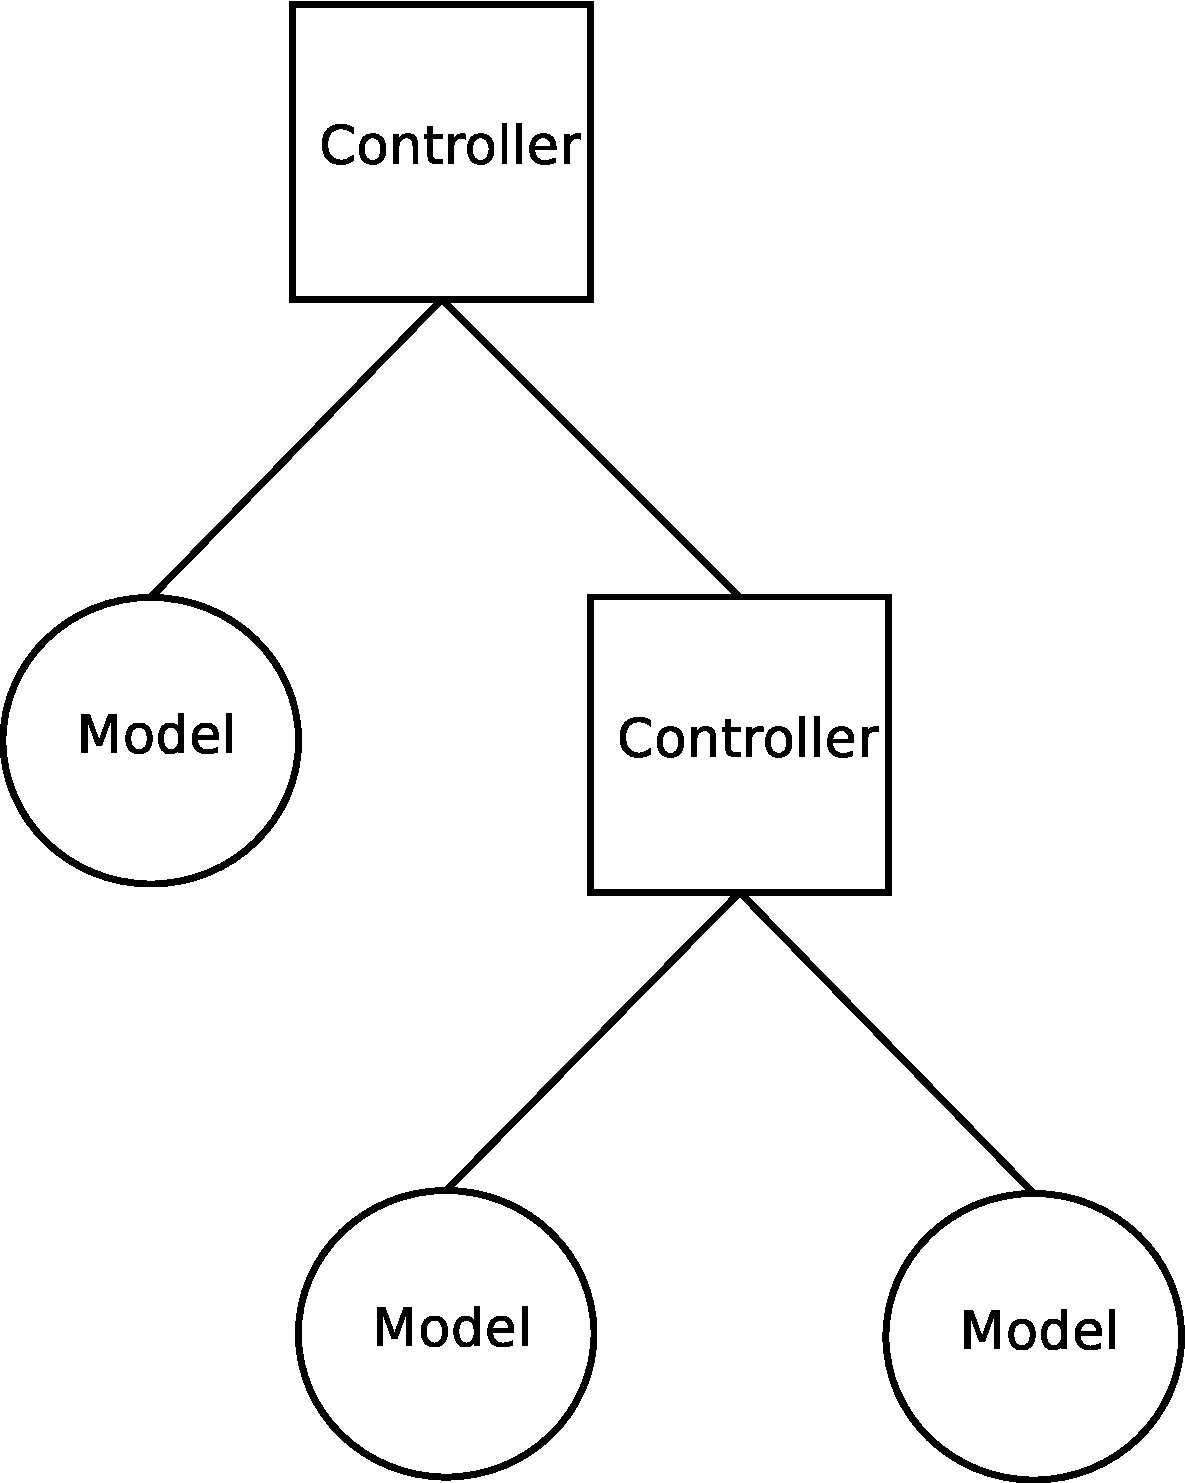
\includegraphics[width=0.75\textwidth]{example_controller_layout.pdf}
\caption{Example controller/model topology}
\label{example_controller_model_topology}
\end{figure}

\subsection{The Utilities}
The utilities module will provide interfaces for data analysis and visualization tools, such as matplotlib, as well as a database on publically available data for commonly modelled componets such as engines and structural beams. It's a catch all module for anything that is useful to modelling and simulation that is not included in the other modules.


\chapter{Detailed Design}
The propsed general design will be tested by implementing a prototype (ESP version 0.1.0, using semantic version numbering), that solves a particular example problem, specifically a 3 degree of freedom (3dof) rocket simulation. The first few iterations of ESP will utilitize this approach.
\section{Version 0.1 Design}
Version 0.1 will implement all of the components of the ESP design necessary to simulate a multistage rocket launch to orbit using a 3 degree of simulation (X,Y,Z position). These components include the following models:
\begin{description}
	\item[Dynamics Model] A simple 3dof simulation of the rocket state and its component parts will intialize at a velocity  and position dictated by the earth's rotation and the rocket's starting lattitude, longitude and altitude. The rocket's position and velocity will then be integrated over time responding to applied forces from gravitational, aerodynamic and engine forces. The rocket's mass will be calculated from a starting mass and a fuel mass that is integrated over time according the the mass flowrate dictated by the engine model.
	\item[Aerodynamics Model] An aerodynamics model will calculate drag on the rocket as a function of Mach number and atmospheric density.
	\item[Atmospheric Model] An atmosphere model will calculate air density according to the rocket's position.
	\item[Gravity Model] A model of the earth's gravitational field and its effects on the rocket.
	\item[Engine Model] A model that calculates thrust from the engines and the direction of that thrust applied to the rocket.
	\item[Engine Controller Model] A model containing the navigation commands (as engine thrust angles) to the rocket. The model will  consist of a set of engine thrust angles at a discrete set of time intervals with cubic splines in between. (Unless theres a better way to do this)
\end{description}
To implement the these models, the following standard module numerical routines and typeswill be implemented:
\begin{description}
	\item[Vector Type] A generic vector type with addition, substraction, dot and cross products and scaling will be implemented. A norm method will also be implemented.
	\item[ODE Solver] An ODE solver will be implemented with interfaces that both return a single time step increment as well as a list of values given a list of time steps. The solver will use the vector type for vectors and generic number types for numbers.
	\item[Unconstrained optimizer] An uncontrained optimizer will be implemented that can optimize the thrust angle nodes.
	\item[Horner's method] Horner's method of evaluating polynomials for quick calculation of the spline values.
	\item[Linear and Quadratic Interpolation] For modelling the engine specific impulse as a function of altitude as well as modelling the atmosphere.
	\item[Cubic splines] For modelling thrust direction.
	\item[Look up tables] For the atmosphere model. 
\end{description}
To coordinate and control these models, the generic, optimization and time modes of the controller program will be implemented. The optimization and time modes will be implemented using models that run last and second to last in a controller cycle. The time mode will be used to advance the time in the dynamics model.

\begin{figure}[h]
\centering
\leavevmode
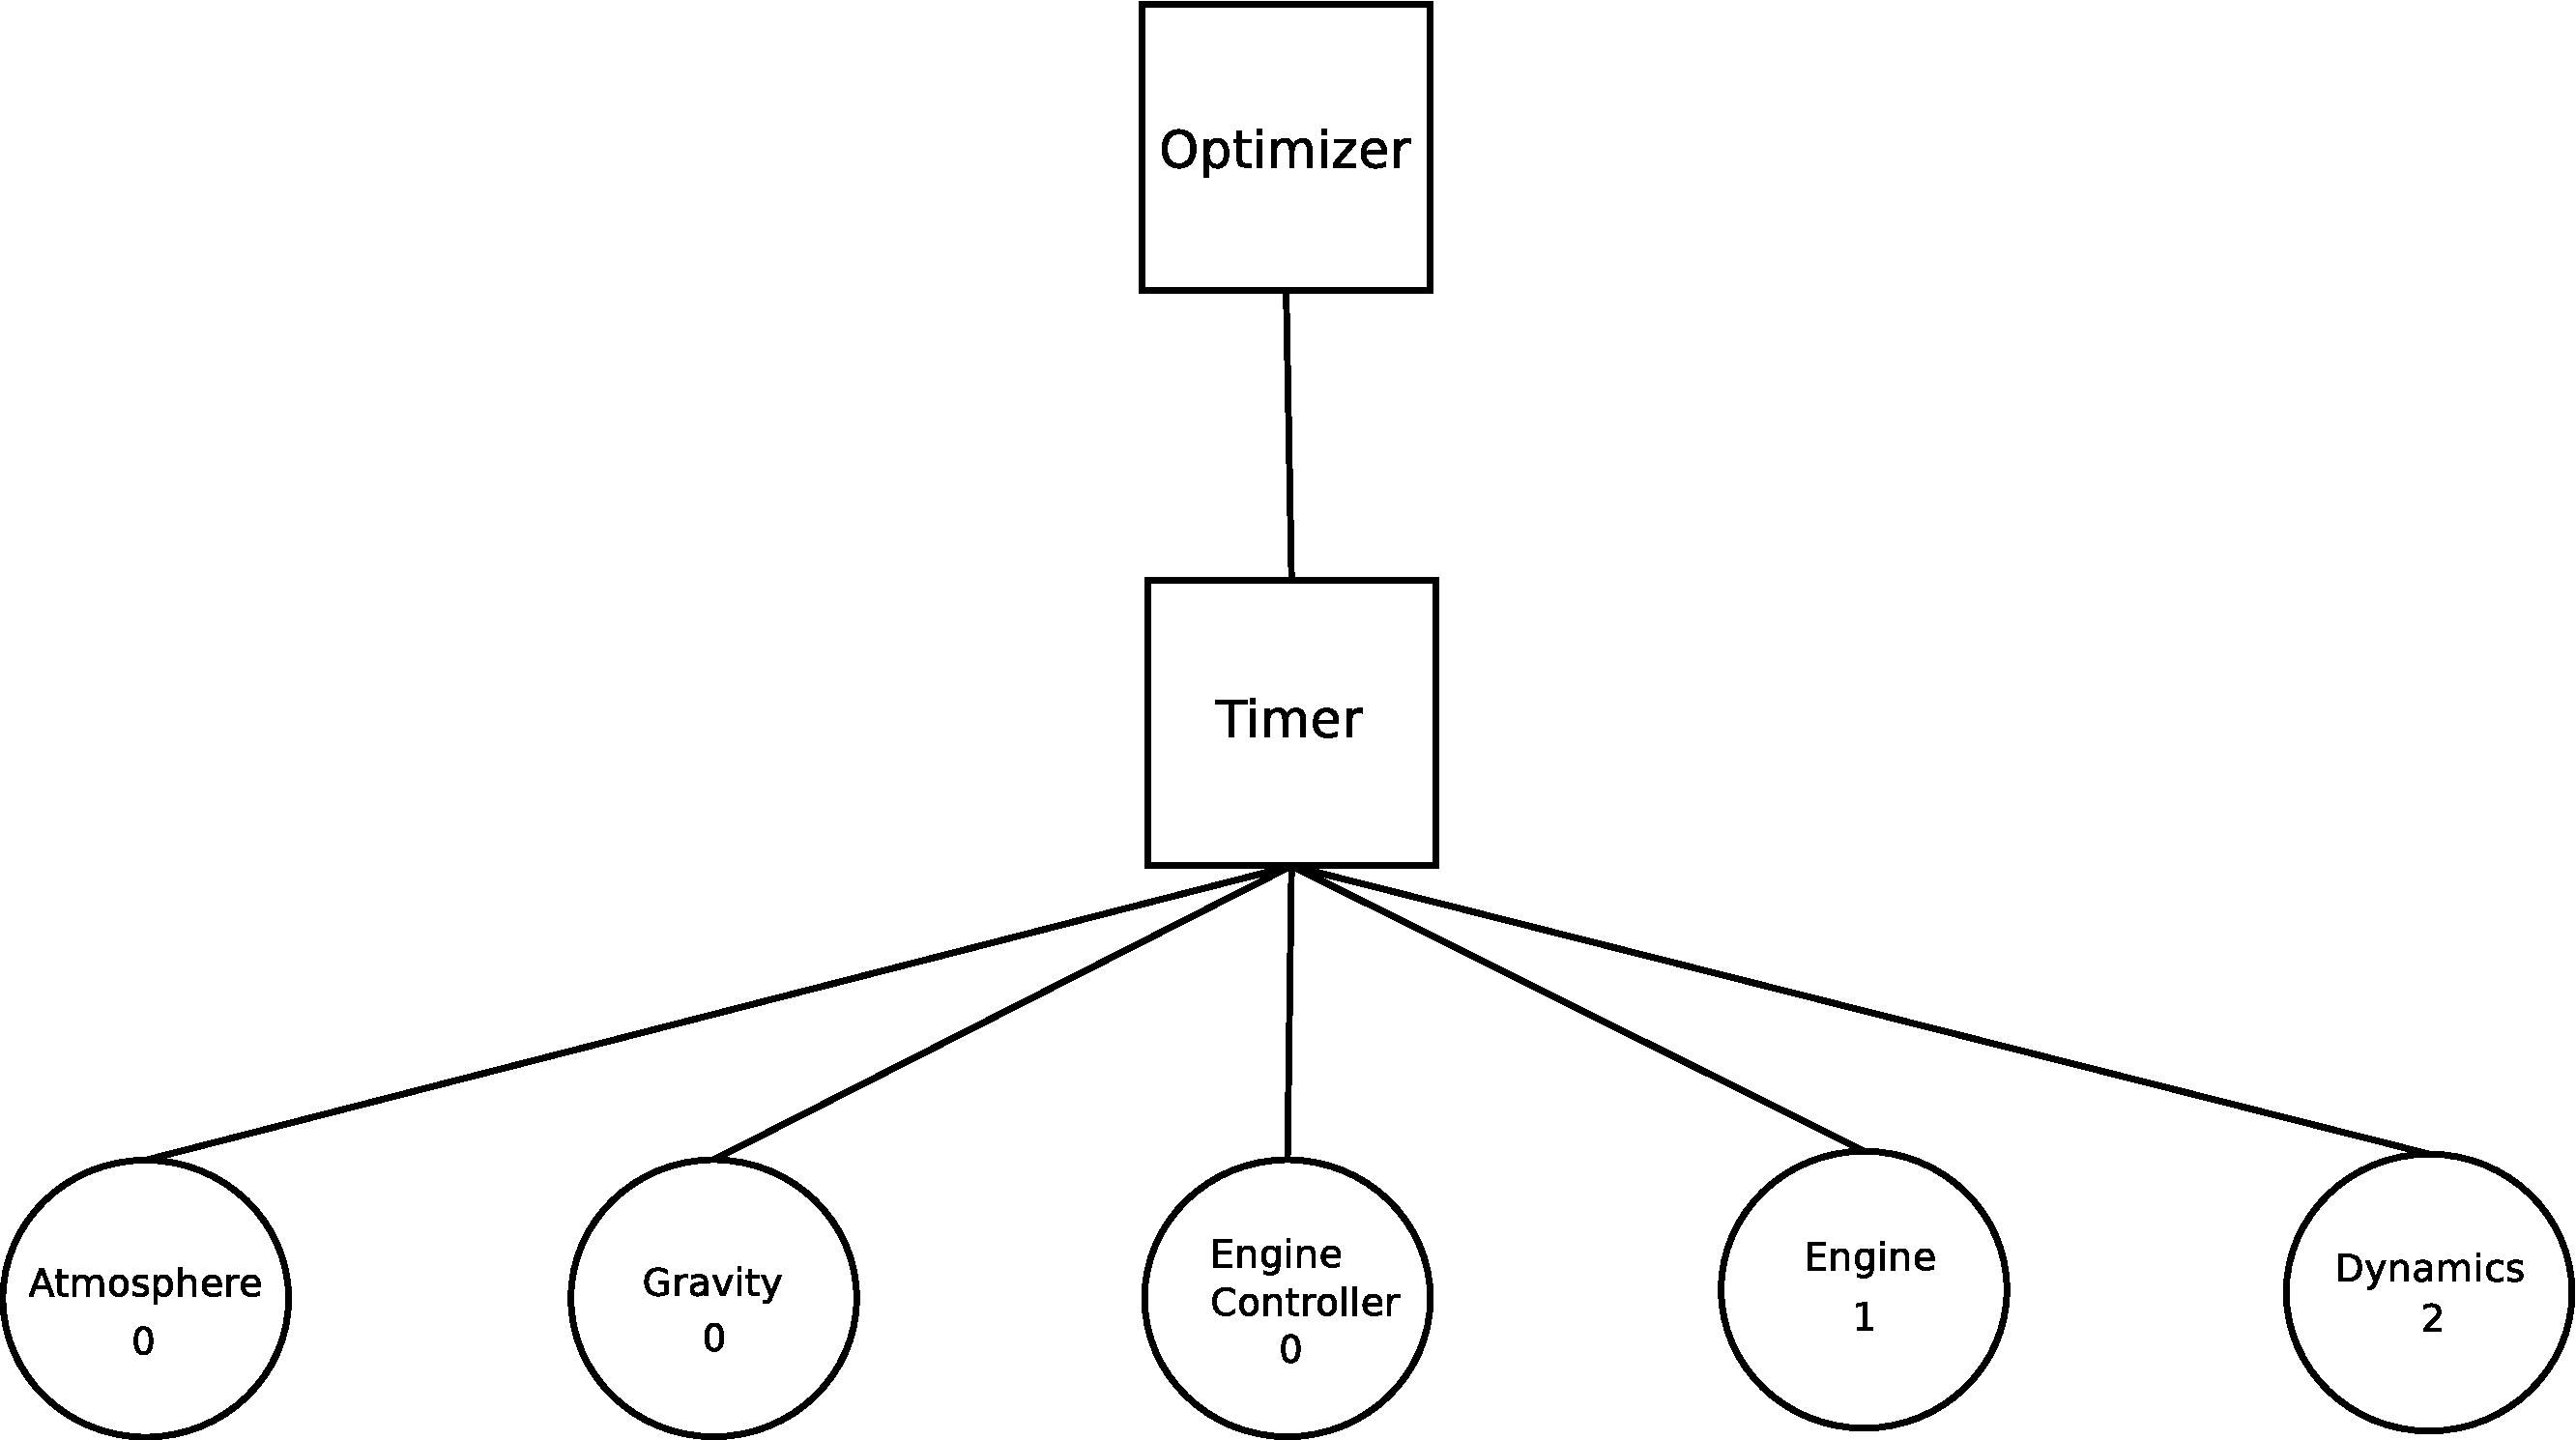
\includegraphics[width=0.75\textwidth]{01layout.pdf}
\caption{Version 0.1 3dof sim topology}
\label{01layout}
\end{figure}

\begin{figure}[h]
\begin{center}
\leavevmode
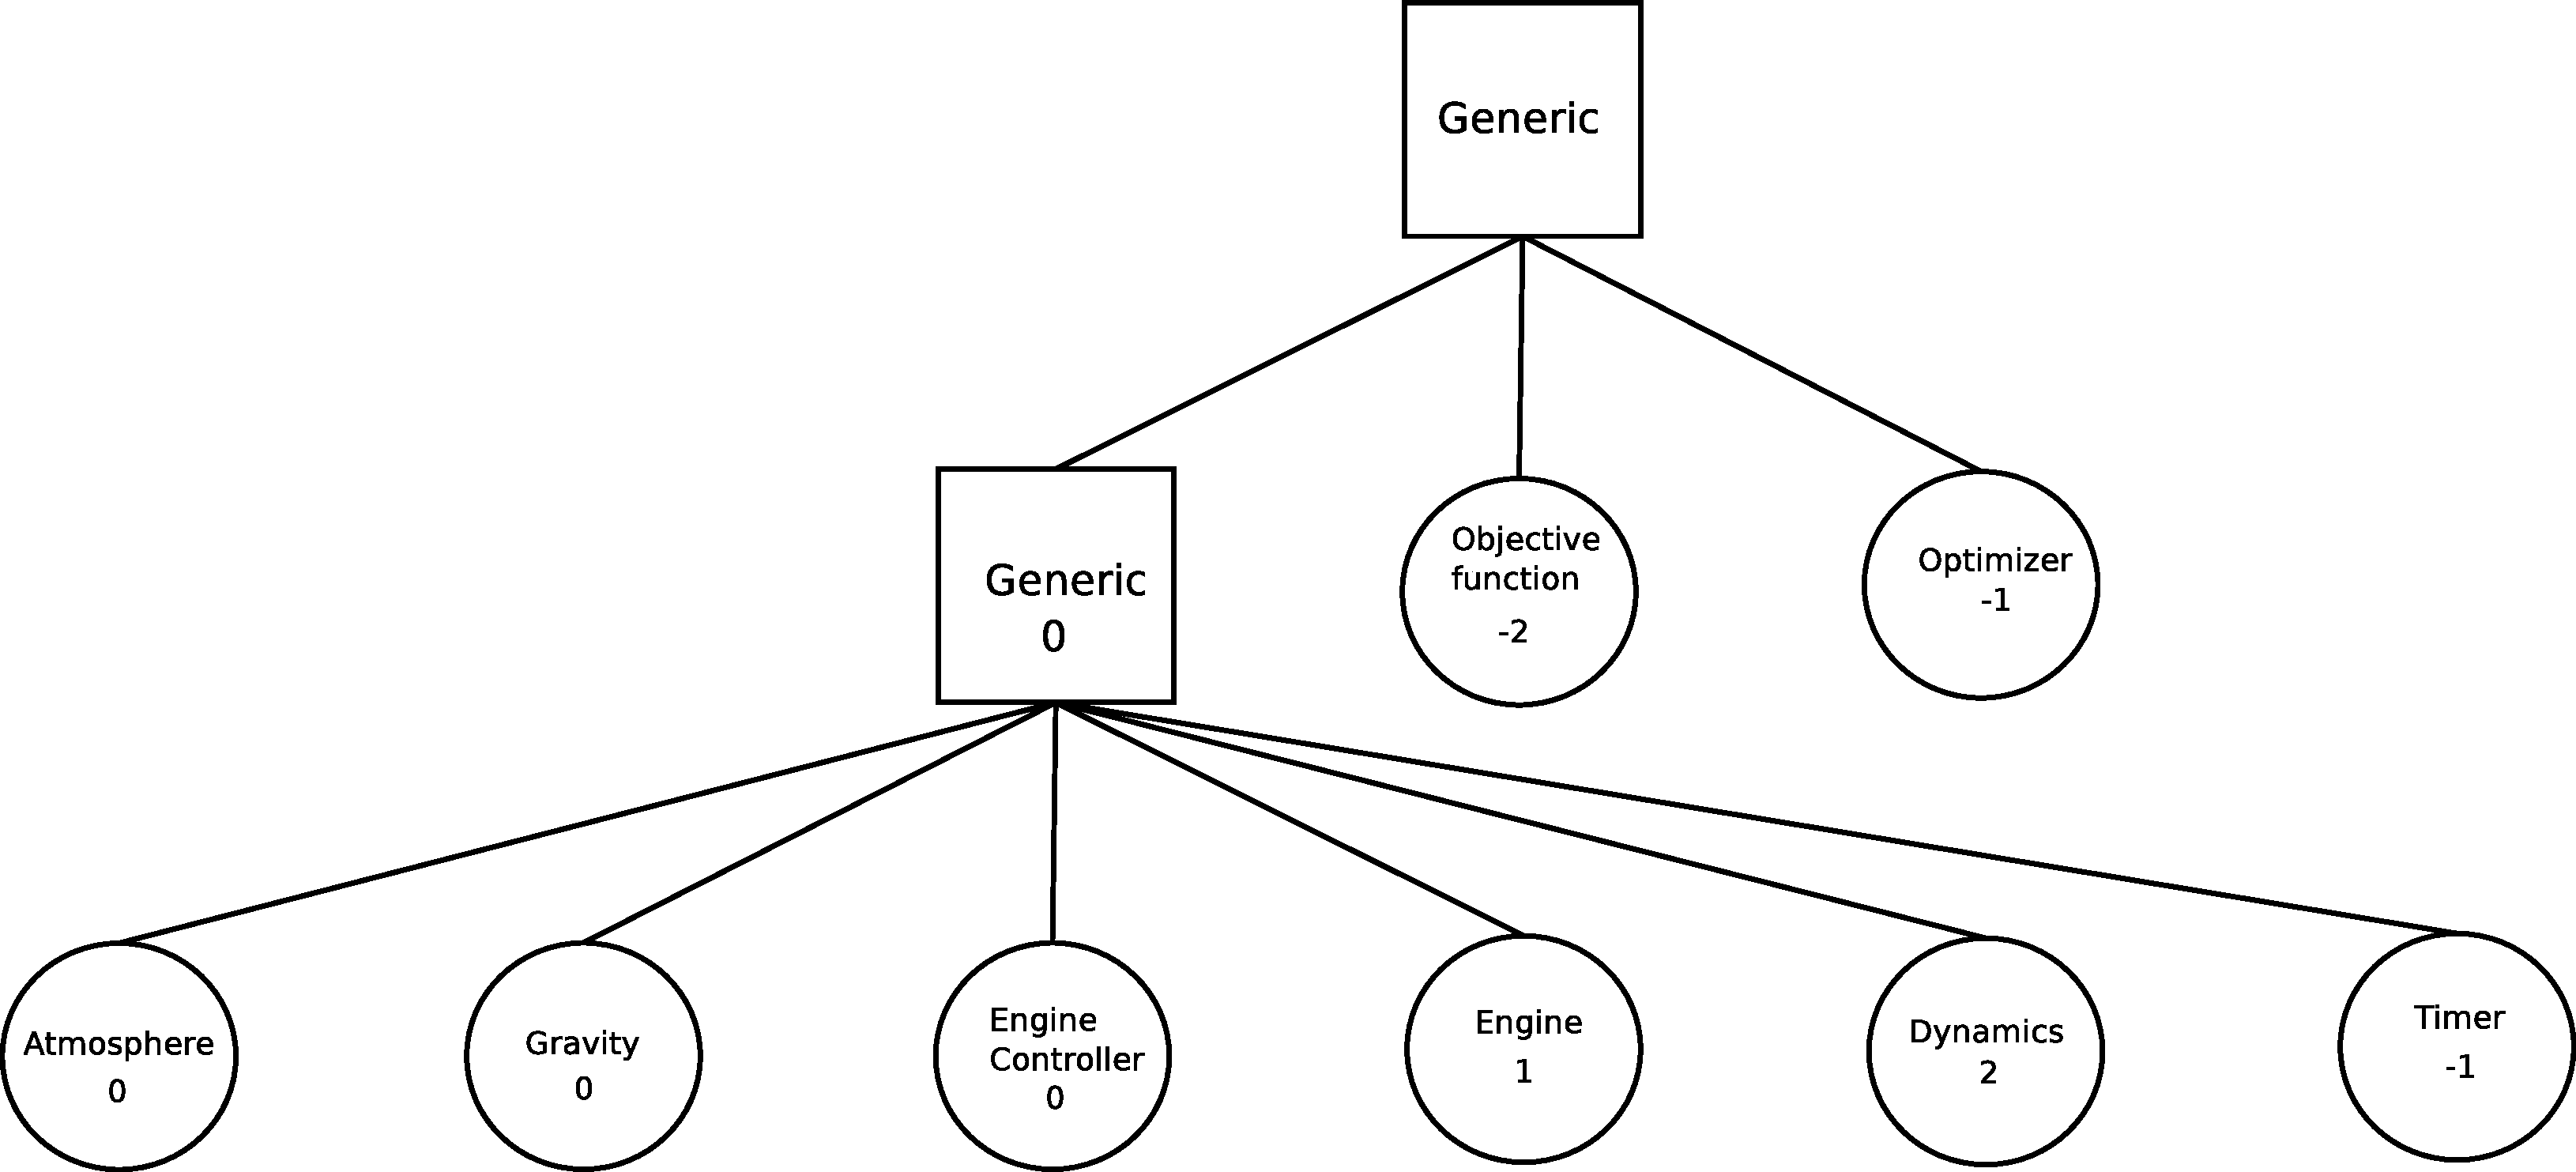
\includegraphics[width=0.75\textwidth]{01layoutalt.pdf}
\end{center}
\caption{Alternate view of 3dof sim topology}
\label{01layout_alt}
\end{figure}

The simulation will be laid out as in Figure~\ref{01layout}. Figure~\ref{01layout_alt} shows the layout of the simulation with the timer, objective function and optimizer models connected to the generic controller programs, explicitly showing how the controller programs will be implemented with respect to the rest of the sim. The numbers are the order numbers which determine the order in which the executables will run.

\section{Run example}

A simulation run consists of starting the root controller program, passing it input via standard in. Then, the children of the controller are started, with input passed in front standard in as well if they are controller programs. A controller program that is not the root passes must first have all of its children register before it registers with its parent. 

Once all of the root node's children have registered, the children can run until they reach controller.get\_inputs(), which should be inside a loop defined using  "while True:". This is the main program loop for the model.  get\_inputs() acts a barrier, so execution pauses until the controller program orders it to proceed. Execution will proceed until it reaches a controller.barrier() or a controller.set\_outputs() call.

controller.barrier() acts as a general purpose barrier and should be used only as a stand in for the get\_inputs() and set\_outputs() calls when no input or output is needed. set\_outputs() sends the model's outputs to the controller program and then pauses execution until the controller program tells it to proceed. Once the last loop is run, exit() can be called from within any of the barrier methods.

Once the root controller sends the shutdown command to its models, it then waits until all the models acknowledge the command before shutting down. Non-root controllers pass the shutdown command to their children and also wait until acknowledgement before both acknowledging their parent's shutdown command and shutting down themselves.

\section{Controller program input commands}

The controller program takes a set of commands, generally passed as file stream, to configure for running the simulation and to be controlled during the run. It may also output status to standard out. There are reserved variable names that should not be used for state variable names: root, cycles, order, run, shutdown, step, status, load.

For the prototype (v0.1) build, we will implement these as python statements.

\begin{description}
	\item[\emph{variable\_name} = \emph{value}] Creates or assigns a \emph{value} to {variable\_name}
	\item[load( \emph{filename} )] Loads a file of controller commands.
	\item[root=\emph{boolean}] Set to True if controller is the root node, False otherwise.
	\item[cycles=\emph{integer}] Number of times the controller will run the loop.
	\item[order[\emph{model\_name}] = \emph{integer} ] The order number of the model named \emph{model\_name}. Defaults to 0.
	\item[run()] Begining running the simulation loop.
	\item[step()] Run on step of the simulation loop.
	\item[shutdown()] Send the shutdown command to children and quit once all acknowledgements have been received.
	\item[state([\emph{name}])] Print the values of the state variable named \emph{name}. Print all of them if no name is given.
	\item[status()] Print the controller program status.
\end{description}

\section{Version 0.1 API}
\begin{alltt}
standard.\textbf{sqrt}(\emph{ argument} )
    Generic square root function that should work on most types. Should try 
    and call class's sqrt method and then default to a generic method.

\emph{class} standard.\textbf{Vector }
    Generic Vector class built on top of lists.

    \textbf{Vector}( \emph{ values [,length] } )
       Vector constructor that takes a list of numbers and returns a Vector.
       If length, a integer, is defined, will return a Vector of \emph{length} elements
       where every element has value \emph{values}. Note that you can create
       vectors of vectors. Vectors of lists and tuples can be created, but mathematical
       operations on them should cause exceptions.

    \textbf{row}
        Boolean set to true if vector is a row vector 
        and false if vector is a column vector

   \textbf{__len__}(\emph{self})
        Returns the number of elements in the vector.

    \textbf{__add__}( \emph{ self, other} )
         Returns a vector that is the sum of self and other.

    \textbf{__sub__}( \emph{ self, other} )
         Returns a vector that is the difference of self and other.

    \textbf{__mul__}( \emph{ self, other} )
         Returns a vector that is the piecewise product of self and other.
         If other is a scalar, multiply it piecewise with self.

    \textbf{__radd__}( \emph{ self, other} )
    \textbf{__rsub__}( \emph{ self, other} )
    \textbf{__rmul__}( \emph{ self, other} )
        The right hand versions of __add__, __sub__ and __mul__.

    \textbf{__getitem__}( \emph{ self, key} )
        Implements assignment from self[key] where key is the 
        index of the element of the vector.

    \textbf{__setitem__}( \emph{ self, key, value} )
        Implements assignment to self[key] where key is the index 
        of the element of the vector.

  \textbf{__repr__}(\emph(self) )
    Implements the evaluatable string representation of the class.

    \textbf{norm}(\emph{self[,p]})
        The norm of the vector (2 norm by default). \emph{p} is
         the p-norm value. No support of infinity yet.

standard.\textbf{norm}(\emph{ vector[,p]})
    The norm of a Vector \emph{vector} (2 norm by default.)
    \emph{p} is the p-norm value. No support of infinity yet.

    Will support other types in future by calling type's norm()
    method.

standard.\textbf{dot}(\emph{ left,right})
    Returns the dot product of left and right.

standard.\textbf{cross}(\emph{ left,right})
    Returns the cross product of left and right.

standard.\textbf{ode_step}(\emph{function, initial_value, step_size[, **kwargs]})
    A single step of an ODE solver. The default choice of solver should 
    be a reasonable explicit, single-step, fixed step solver such as RK4. 
    \emph{function} should be a  function x'=f( x,t ) such that x is a 
    scalar or Vector and t is a real scalar and x' is
    the derivative of x with respect to t.

    \emph{initial_value} is the initial value of the function at the
     start time, which defaults to t=0. \emph{step_size} is the 
     initial time step size. 

    The \emph{**kwargs} arguments will allow the user to select
    different solvers, different solver options and to pass 
    previous time step data to multistep methods.

standard.\textbf{ode_solve}(\emph{function, initial_value, steps[, **kwargs]})
    An ODE solver that repeated applies \emph{ode_step}() to \emph{function}.
    The inputs are the same as \emph{ode_step}() except that instead of \emph{step_size},
    \emph{steps} takes a list of times and solves for those times. If a variable time step 
    method is used, \emph{steps} should be a 3-tuple 
    (intial time, intial step size, final time)

standard.\textbf{optimize}(\emph{function, initial_value[, **kwargs]})
    A gradient based optimizer that begins at \emph{intial_value} and 
    searches for a local optimum. \emph{function} should be a
    function y=f( x ) such that x is a Vector and y is a scalar objective 
    function.

    Any necessary options are passed via \emph{kwargs} and
    constraints are not supported yet.

standard.\textbf{horners_method}(\emph{coefficients[, argument]})
    Returns a function that takes a value x and returns 
    the value of the polynomial with Horner's method coefficents
    \emph{coefficients}. If \emph{argument} is given, then 
    \textbf{horners_method}() returns the value of the polynomial
    instead of a function.

standard.\textbf{interpolate}(\emph{points [, value, **kwargs ]} )
    Returns a function that gives the interpolation between points
    \emph{points}. Only supports 1 dimensional interpolation currently.
    If \emph{value} is given, returns the value of the interpolation rather
    than a function.

    \emph{**kwargs} allows setting options, currently \emph{type=}
    either "linear", "quadratic" or "spline". Linear interpolation is the default, and
    should only require 2 points while quadratic interpolation will require
    3 points.
	
\emph{class} standard.\textbf{LookupTable }
    Lookup table class. Currently, 1 dimensional only. Provides
    nearest neighbor lookup, linear and quadratic interpolation
    and cubic spline approximation. 

  \textbf{LookupTable}(\emph{[table]} )
      Default constructor that initializes lookup table. If 
      a dictionary \emph{table} is provided whose keys are
      a non repeating orderable list, the keys become the
      independent variables and the values become the dependent
      variables.

  \textbf{load}(self,fileid)
      Load a lookup table from file stream \emph{fileid}.

  \textbf{lookup}(self,argument, method="linear")
      Look up the approximate value of the function
      described by lookup table for the chosen method
      and the given argument. \emph{method} may have
      values of "linear", "neighbor","quadratic","spline"

  \textbf{functionfy}(self,method="linear")
      Return a function y = f(x) that wraps the lookup table lookup()
      by returning a value y for a given x.

  \textbf{__getitem__}(self,key)
      Return the dependent variable value associated with \emph{key}.
      If there isn't one, return None.

  \textbf{__setitem__}(self,key)
      Set the dependent variable value associated with \emph{key}.

\emph{class} standard.models.ase.\textbf{RocketEngine}
  A rocket engine class that contains lookup tables for exhaust
  velocity  as a function of ambient pressure and propellant 
  flowrate as a function of throttle command.

  \textbf{flowrate_table} 
    A LookupTable for thrust as function of throttle command.

  \textbf{exhaust_velocity_table}
    A LookupTable for exhaust velocity as a function of ambient
    pressure.

  \textbf{load}(\emph{file_id})
    Load the engine's lookup tables from file stream \emph{file_id}.

  \textbf{flowrate}(\emph{throttle})
    Function that returns flowrate given a real throttle input.

  \textbf{exhaust_velocity}(\emph{ambient_pressure})
    Function that returns an exhaust velocity given an ambient
    pressure.

  \textbf{thrust}(\emph{throttle, ambient_pressure})
    Function that returns thrust given ambient pressure
    and throttle.

\emph{class} standard.models.ase.\textbf{Atmosphere}
  A class that models the atmosphere.

  \textbf{density}(\emph{altitude} )
    A function that returns density as a function of altitude.

  \textbf{pressure}(\emph{altitude} )
    A function that returns pressure as a function of altitude.

  \textbf{speed_of_sound}(\emph{altitude} )
    A function that returns speed of sound as a function of altitude.

\emph{class} standard.models.ase.\textbf{Gravity}
  A class that models the Earth's gravitational field.

  \textbf{little_g}(\emph{location, [sideral_time] } )
    Returns a vector of the locale gravitational acceleration for
    \emph{location}. \emph{location} is assumed to be ECF
    frame if no sideral time is given and in ECI inertial if sideral time
    is given.

  \textbf{potential}(\emph{location, [sideral_time] } )
    Returns the local gravitational potential for
    \emph{location}. \emph{location} is assumed to be ECF
    frame if no sideral time is given and in ECI inertial if sideral time
    is given.

\emph{class} standard.models.ase.\textbf{Aerodynamics}
  Class modeling drag on the rocket. Uses a look table that
  estimates coefficient of drag as a function of Mach number.
  Utilizes an atmosphere model.

  \textbf{load}(\emph{file_id})
    Loads coefficient of drag table from file stream \emph{file_id}

  \textbf{set_atmosphere}(\emph{atmosphere})
    Sets aero model's atmosphere to the \emph{atmosphere}
    object.

  \textbf{mach_number}(\emph{ altitude, speed})
    Returns Mach number given the altitude and
    object's speed.

  \textbf{drag_coefficient}(\emph{mach_number})
    Returns drag coefficient given a Mach number.

  \textbf{drag_force}(\emph{mach_number, altitude, ref_area})
    Returns a drag force vector given a Mach number, altitude and
    a reference area.

\emph{class} standard.models.ase.\textbf{EngineController}
  Class that implements open loop guidance via engine angles 
  as rotations about the x (theta) and y (phi) axes of the 
  ECI reference frame as functions of time.

  \textbf{theta}(\emph{time})
    Returns the engine thrust line angle about the ECI x axis as a 
    function of time.

  \textbf{phi}(\emph{time})
    Returns the engine thrust line angle about the ECI y axis as a 
    function of time.

controller.\textbf{register}( \emph{name, location} )
  Register this model as \emph{name} with controller program at 
  location \emph{location}

controller.\textbf{get_inputs}( state_names )
  Returns a dictionary with the members of \emph{state_names}
  list as keys and the values of those states as their values. The states
  are those maintained by the controller program. The names of the states
  are known to the model and the control program (and can be ints, str, etc).
  Also acts as barrier. Execution proceeds after the controller program orders 
  it to continue.

controller.\textbf{set_outputs}( state_dictionary )
  Sends the global state in \emph{state_dictionary} back to the controller
  program the model is registered with. This also acts a barrier, waiting on
  the controller program to order continued execution.

controller.\textbf{barrier}()
  A barrier that pauses model execution until the controller program tells it
  to continue.

controller.\textbf{rewind}(\emph{ state_dictionary })
  Request that the controller program rerun the previous iteration using
  the state from that iteration with only the states in \emph{state_dictionary}

controller.\textbf{shutdown}()
  Request the that controller program send a shutdown command to the models.

controller.\textbf{running}()
  Returns True if the controller program has not sent the shutdown command and
  False if it has.

\end{alltt}

\end{document}